% Options for packages loaded elsewhere
\PassOptionsToPackage{unicode}{hyperref}
\PassOptionsToPackage{hyphens}{url}
%
\documentclass[
]{book}
\usepackage{amsmath,amssymb}
\usepackage{lmodern}
\usepackage{iftex}
\ifPDFTeX
  \usepackage[T1]{fontenc}
  \usepackage[utf8]{inputenc}
  \usepackage{textcomp} % provide euro and other symbols
\else % if luatex or xetex
  \usepackage{unicode-math}
  \defaultfontfeatures{Scale=MatchLowercase}
  \defaultfontfeatures[\rmfamily]{Ligatures=TeX,Scale=1}
\fi
% Use upquote if available, for straight quotes in verbatim environments
\IfFileExists{upquote.sty}{\usepackage{upquote}}{}
\IfFileExists{microtype.sty}{% use microtype if available
  \usepackage[]{microtype}
  \UseMicrotypeSet[protrusion]{basicmath} % disable protrusion for tt fonts
}{}
\makeatletter
\@ifundefined{KOMAClassName}{% if non-KOMA class
  \IfFileExists{parskip.sty}{%
    \usepackage{parskip}
  }{% else
    \setlength{\parindent}{0pt}
    \setlength{\parskip}{6pt plus 2pt minus 1pt}}
}{% if KOMA class
  \KOMAoptions{parskip=half}}
\makeatother
\usepackage{xcolor}
\usepackage{longtable,booktabs,array}
\usepackage{calc} % for calculating minipage widths
% Correct order of tables after \paragraph or \subparagraph
\usepackage{etoolbox}
\makeatletter
\patchcmd\longtable{\par}{\if@noskipsec\mbox{}\fi\par}{}{}
\makeatother
% Allow footnotes in longtable head/foot
\IfFileExists{footnotehyper.sty}{\usepackage{footnotehyper}}{\usepackage{footnote}}
\makesavenoteenv{longtable}
\usepackage{graphicx}
\makeatletter
\def\maxwidth{\ifdim\Gin@nat@width>\linewidth\linewidth\else\Gin@nat@width\fi}
\def\maxheight{\ifdim\Gin@nat@height>\textheight\textheight\else\Gin@nat@height\fi}
\makeatother
% Scale images if necessary, so that they will not overflow the page
% margins by default, and it is still possible to overwrite the defaults
% using explicit options in \includegraphics[width, height, ...]{}
\setkeys{Gin}{width=\maxwidth,height=\maxheight,keepaspectratio}
% Set default figure placement to htbp
\makeatletter
\def\fps@figure{htbp}
\makeatother
\setlength{\emergencystretch}{3em} % prevent overfull lines
\providecommand{\tightlist}{%
  \setlength{\itemsep}{0pt}\setlength{\parskip}{0pt}}
\setcounter{secnumdepth}{5}
\usepackage{booktabs}
\usepackage{amsthm}
\makeatletter
\def\thm@space@setup{%
  \thm@preskip=8pt plus 2pt minus 4pt
  \thm@postskip=\thm@preskip
}
\makeatother
\ifLuaTeX
  \usepackage{selnolig}  % disable illegal ligatures
\fi
\usepackage[]{natbib}
\bibliographystyle{apalike}
\IfFileExists{bookmark.sty}{\usepackage{bookmark}}{\usepackage{hyperref}}
\IfFileExists{xurl.sty}{\usepackage{xurl}}{} % add URL line breaks if available
\urlstyle{same} % disable monospaced font for URLs
\hypersetup{
  pdftitle={Bookdown - Grupo B},
  pdfauthor={Andrés Peralta Alean, David Barrera Barrera, Luis Gonzalo Guerra J},
  hidelinks,
  pdfcreator={LaTeX via pandoc}}

\title{Bookdown - Grupo B}
\author{Andrés Peralta Alean, David Barrera Barrera, Luis Gonzalo Guerra J}
\date{2023-05-22}

\begin{document}
\maketitle

{
\setcounter{tocdepth}{1}
\tableofcontents
}
\hypertarget{propuesta}{%
\chapter{Propuesta}\label{propuesta}}

Análisis de riesgo crediticio y su importancia La evaluación del riesgo crediticio es una tarea crítica para cualquier empresa que ofrezca préstamos o créditos.
El incumplimiento de los términos del préstamo o la falta de pago pueden generar grandes pérdidas financieras y afectar la estabilidad de la empresa.
Es por ello que es importante contar con herramientas y técnicas que permitan evaluar el riesgo crediticio de manera eficiente.

El análisis de riesgo crediticio utiliza históricos para evaluar el comportamiento de los clientes a lo largo de varios periodos.
De esta forma, se pueden obtener patrones y características que permiten segregar grupos de clientes y determinar un posible perfil de riesgo.
Los resultados obtenidos a partir de este análisis pueden ayudar a la empresa a tomar decisiones más informadas y a reducir el riesgo crediticio.

Además, el análisis de riesgo crediticio permite identificar posibles oportunidades para la empresa.
Por ejemplo, puede ayudar a la empresa a identificar clientes que presenten un bajo riesgo crediticio y, por lo tanto, puedan recibir préstamos con tasas de interés más bajas.
De esta manera, la empresa puede aumentar su base de clientes y mejorar su rentabilidad.

En cuanto a las fuentes de información, se pueden utilizar diversas fuentes para recopilar los datos necesarios para el análisis de riesgo crediticio.
Entre ellas se encuentran bases de datos públicas y privadas, encuestas, registros gubernamentales, entre otras.
Es importante verificar la calidad de la información obtenida para asegurar la precisión y confiabilidad de los resultados.

En el caso específico de la empresa ABC, se cuenta con los permisos necesarios por parte del área de gestión de cobranzas y se eliminaron los datos personales de los clientes con los cuales se extrajeron las características.

En resumen, el análisis de riesgo crediticio es una técnica muy útil para evaluar el riesgo crediticio de los clientes y para identificar posibles oportunidades para la empresa.
Se pueden utilizar diversas fuentes de información para recopilar los datos necesarios para este análisis, pero es importante asegurarse de contar con los permisos necesarios y verificar la calidad de la información obtenida.

\hypertarget{Analisis}{%
\chapter{Analisis Exploratorio}\label{Analisis}}

\hypertarget{introducciuxf3n}{%
\section{Introducción}\label{introducciuxf3n}}

En este análisis, se explorará el comportamiento de la utilización de los productos de un banco a lo largo de los años. Se examinará si ha habido un incremento en la utilización de los productos año a año, y en caso afirmativo, se intentará identificar cuáles son las razones que han llevado a este aumento.

En particular, se examinará la utilización de los productos de un banco desde el año 2018 hasta el año en curso. Se considerarán productos tales como tarjetas de crédito y crédito de consumo. Se investigará si existe un patrón estacional en la utilización de estos productos, es decir, si hay un comportamiento cíclico que se repite en determinados meses del año. Además, se estudiará la posible existencia de tendencias a largo plazo que puedan indicar un cambio en el comportamiento de los clientes del banco y que posibles factores indicen en estos cambios.

La metodología utilizada en este análisis incluye la descomposición de series de tiempo, la identificación de patrones estacionales y la realización de pruebas estadísticas para verificar la presencia de tendencias y cambios en el comportamiento de los clientes.

\hypertarget{explicaciuxf3n-de-la-base}{%
\section{Explicación de la base}\label{explicaciuxf3n-de-la-base}}

Partimos de una base agrupada con las siguientes variables:

Periodo - \textgreater{} año y mes
Sub\_Tipo -\textgreater{} tipo de producto
N\_Clientes -\textgreater{} cantidad de cleintes
DIAS\_DE\_MORA -\textgreater{} días de mora de los clientes a cierre de mes
Saldo -\textgreater{} saldo utilizado por los clientes a cierre de mes
Genero -\textgreater{} genero del cliente
grupo\_actividad\_eco -\textgreater{} que actividad económica tiene el grupo de clienes
Cuidad\_res -\textgreater{} ciudad de residencia de los clientes

\hypertarget{creacion-del-objeto-de-analisis-temporal-indice.ts}{%
\section{Creacion del objeto de analisis temporal indice.ts}\label{creacion-del-objeto-de-analisis-temporal-indice.ts}}

\hypertarget{carga-de-librerias-y-datasource}{%
\subsection{Carga de librerias y datasource}\label{carga-de-librerias-y-datasource}}

\begin{verbatim}
## Registered S3 method overwritten by 'quantmod':
##   method            from
##   as.zoo.data.frame zoo
\end{verbatim}

\begin{verbatim}
## Loading required package: zoo
\end{verbatim}

\begin{verbatim}
## 
## Attaching package: 'zoo'
\end{verbatim}

\begin{verbatim}
## The following objects are masked from 'package:base':
## 
##     as.Date, as.Date.numeric
\end{verbatim}

\begin{verbatim}
## Successfully loaded changepoint package version 2.2.4
##  See NEWS for details of changes.
\end{verbatim}

\begin{verbatim}
## # A tibble: 643,570 x 8
##    Periodo Sub_Tipo N_Clientes DIAS_DE_MORA     Saldo Genero grupo_actividad_eco
##    <chr>   <chr>         <dbl>        <dbl>     <dbl> <chr>  <chr>              
##  1 2018-01 CDC               4            0 15824105. Femen~ Dependiente privado
##  2 2018-01 CDC               1            0  6810373. Femen~ Dependiente privado
##  3 2018-01 CDC               6            6 28819502. Femen~ Dependiente privado
##  4 2018-01 CDC              12           63 81343674. Femen~ Dependiente privado
##  5 2018-01 CDC               1           21  7524344. Femen~ Dependiente privado
##  6 2018-01 CDC               4            0 12974213. Femen~ Dependiente privado
##  7 2018-01 CDC               3            1 21348609. Femen~ Dependiente privado
##  8 2018-01 CDC               2            0 11475858. Femen~ Dependiente privado
##  9 2018-01 CDC              10           38 60012355. Femen~ Dependiente privado
## 10 2018-01 CDC               1            0  9034715. Femen~ Dependiente privado
## # i 643,560 more rows
## # i 1 more variable: Cuidad_res <chr>
\end{verbatim}

\hypertarget{modificamos-el-df-para-que-tenga-el-formato-adecuado-y-lo-mostramos}{%
\subsection{Modificamos el df para que tenga el formato adecuado y lo mostramos}\label{modificamos-el-df-para-que-tenga-el-formato-adecuado-y-lo-mostramos}}

\begin{verbatim}
##               Jan          Feb          Mar          Apr          May
## 2018 2.562223e+12 2.601532e+12 2.653315e+12 2.717915e+12 2.852608e+12
## 2019 3.732137e+12 3.810740e+12 3.923380e+12 3.995810e+12 4.092819e+12
## 2020 2.022405e+12 4.295886e+12 4.304185e+12 4.195404e+12 4.177219e+12
## 2021 4.369300e+12 4.478002e+12 4.595047e+12 4.627874e+12 4.705783e+12
## 2022 6.351501e+12 6.555819e+12 6.739823e+12 6.925001e+12 7.132542e+12
## 2023 8.083445e+12 7.951094e+12 7.812947e+12 7.765132e+12             
##               Jun          Jul          Aug          Sep          Oct
## 2018 2.986446e+12 3.102493e+12 3.196138e+12 3.272388e+12 3.394038e+12
## 2019 4.164386e+12 4.198177e+12 4.267921e+12 4.307340e+12 4.113506e+12
## 2020 4.164434e+12 4.082507e+12 4.067948e+12 4.120926e+12 4.182877e+12
## 2021 4.846473e+12 4.983882e+12 5.091594e+12 5.385784e+12 5.730839e+12
## 2022 7.435792e+12 7.529328e+12 7.670212e+12 7.789046e+12 7.903472e+12
## 2023                                                                 
##               Nov          Dec
## 2018 3.617129e+12 3.690229e+12
## 2019 4.314034e+12 4.455499e+12
## 2020 4.344709e+12 4.384188e+12
## 2021 5.955740e+12 6.164705e+12
## 2022 8.115444e+12 8.154174e+12
## 2023
\end{verbatim}

Deacuerdo al analisis que deseamos hacer consolidamos nuestra variable de interes saldo agrupandola por periodo de tiempo y procedimos a graficar

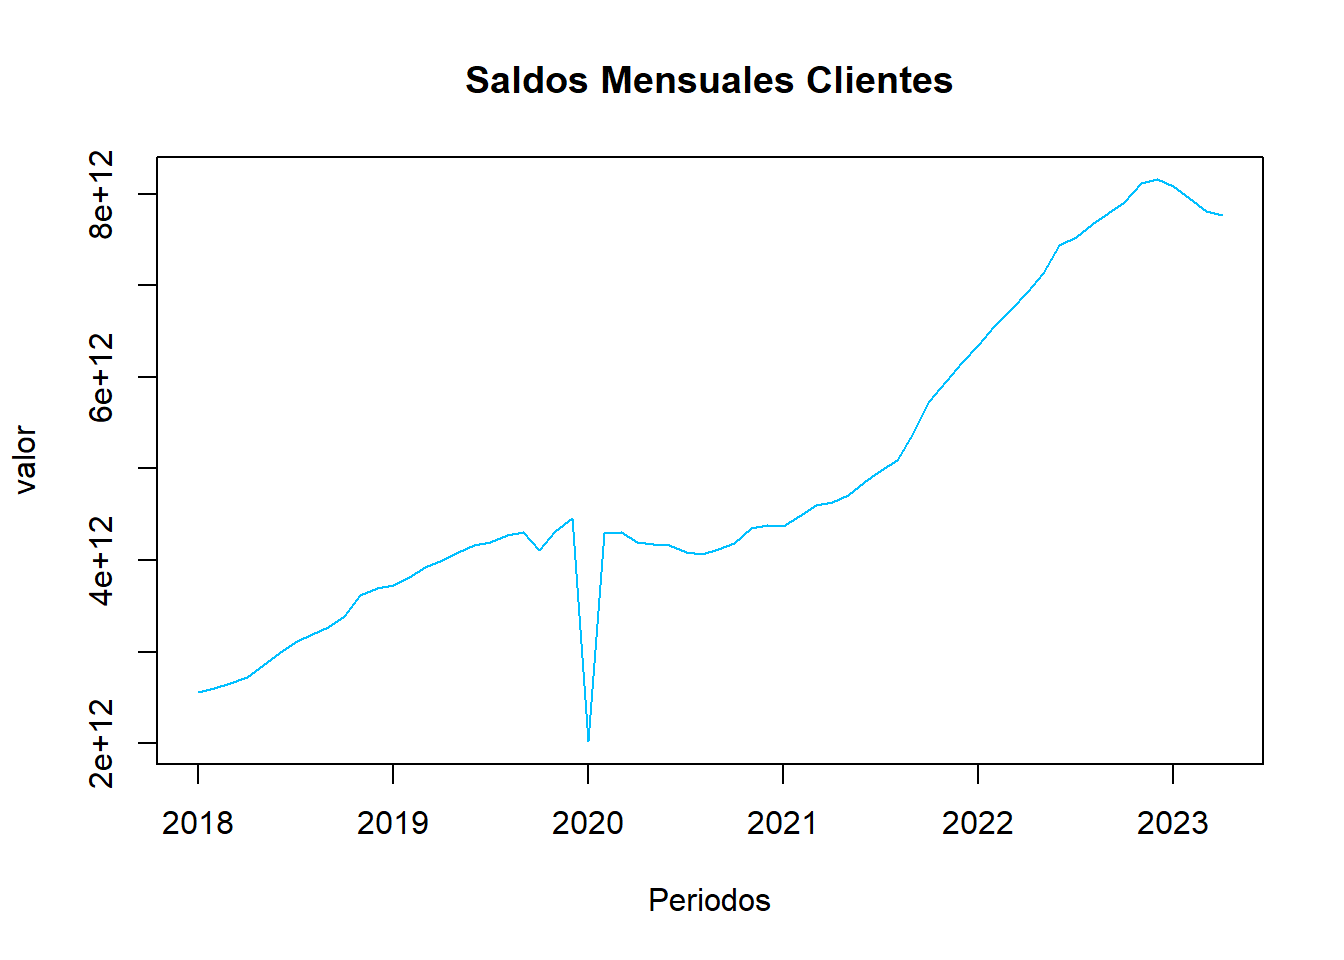
\includegraphics{bookdown-demo_files/figure-latex/unnamed-chunk-3-1.pdf}

\hypertarget{analisis-grafica-de-serie}{%
\subsection{Analisis Grafica de serie}\label{analisis-grafica-de-serie}}

Después de graficar la serie de tiempo, podemos observar ciertas características que nos brindan información valiosa. Por ejemplo, en el primer periodo del 2020, podemos notar un pico descendente en el saldo, lo que podría sugerir un posible error en el registro de los datos históricos.

Por otro lado, al examinar el comportamiento general de la serie de tiempo, se observa un aumento en la utilización de los productos a lo largo de los años, especialmente marcado a partir de la mitad del 2020. Este aumento podría deberse a factores como la pandemia y el desempleo, que podrían haber influido en la demanda de estos productos.

\hypertarget{chequeos-basicos-para-confirmar-la-estructura-del-contenedor-ts}{%
\subsection{Chequeos basicos para confirmar la estructura del contenedor ts}\label{chequeos-basicos-para-confirmar-la-estructura-del-contenedor-ts}}

\begin{verbatim}
## [1] "El tipo de datos del df indice.ts es: "
\end{verbatim}

\begin{verbatim}
## [1] "ts"
\end{verbatim}

\begin{verbatim}
## [1] "La serie de tiempo indice.ts empieza en: "
\end{verbatim}

\begin{verbatim}
## [1] 2018    1
\end{verbatim}

\begin{verbatim}
## [1] "La serie de tiempo indice.ts termina en: "
\end{verbatim}

\begin{verbatim}
## [1] 2023    4
\end{verbatim}

\hypertarget{analisis-descriptivo}{%
\section{Analisis Descriptivo}\label{analisis-descriptivo}}

\hypertarget{grafica-de-rezagos}{%
\subsection{Grafica de Rezagos}\label{grafica-de-rezagos}}

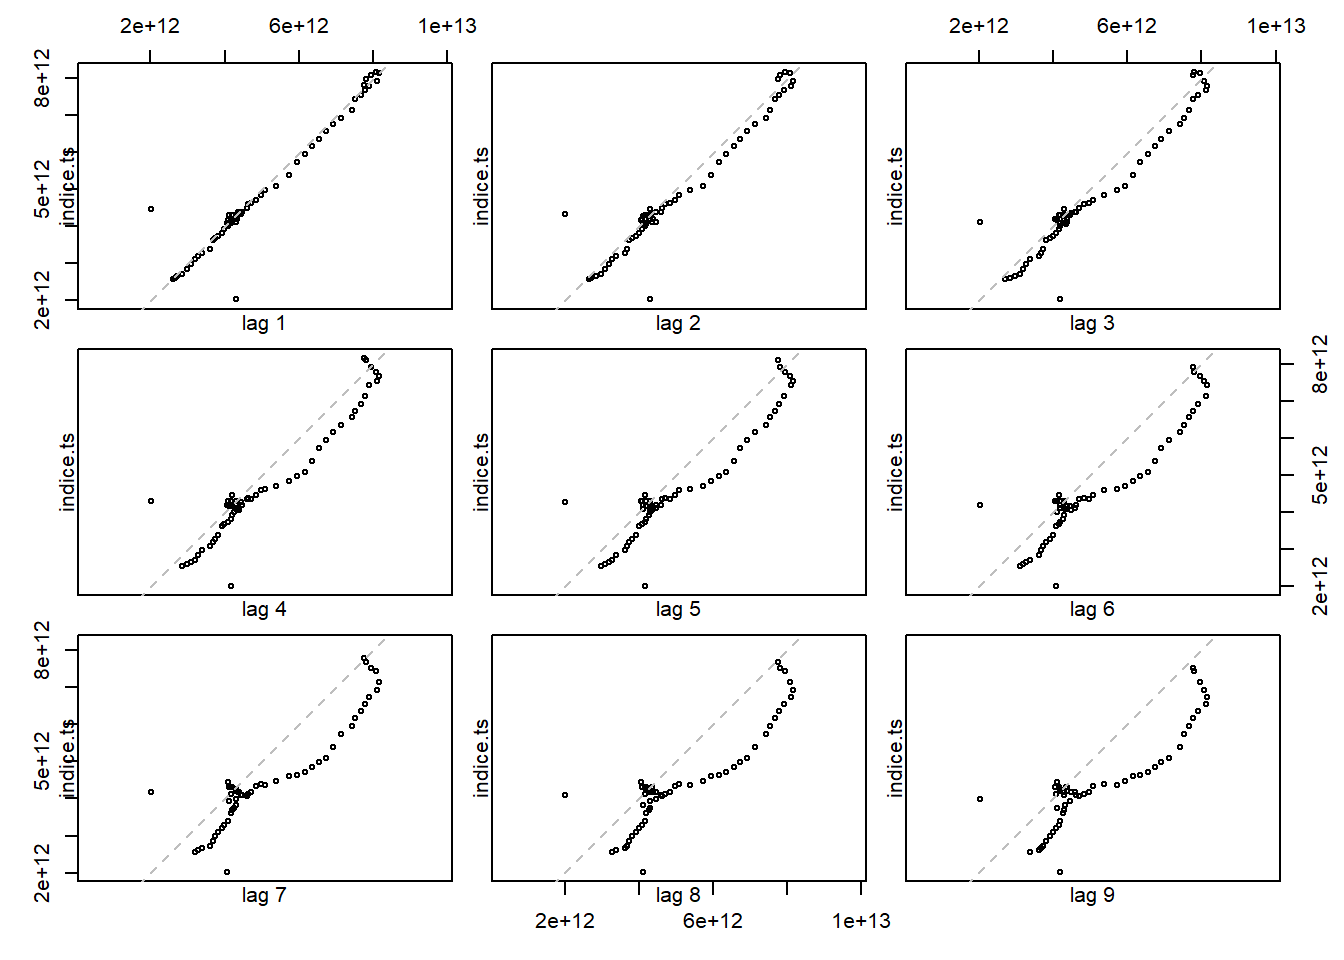
\includegraphics{bookdown-demo_files/figure-latex/unnamed-chunk-5-1.pdf}
Conclusion: Se observa con claridad que existe una tendencia positiva. Esto sugiere una posible transformacion en una etapa posterior del analisis.

\hypertarget{media-movil}{%
\subsection{Media Movil}\label{media-movil}}

Crearemos a continuacion 3 medias moviles para el objeto ts. Estas tendran 3, 5 y 7 periodos para su calculo.

\begin{verbatim}
## Media Movil con 3 meses:  2.60569e+12 2.657587e+12 2.741279e+12 2.852323e+12 2.980516e+12 3.095026e+12 3.19034e+12 3.287521e+12 3.427851e+12 3.567132e+12 3.679831e+12 3.744369e+12 3.822086e+12 3.909977e+12 4.004003e+12 4.084338e+12 4.151794e+12 4.210161e+12 4.257812e+12 4.229589e+12 4.24496e+12 4.294346e+12 3.597313e+12 3.591264e+12 3.540826e+12 4.265159e+12 4.225603e+12 4.179019e+12 4.141387e+12 4.104963e+12 4.090461e+12 4.123917e+12 4.216171e+12 4.303925e+12 4.366066e+12 4.410497e+12 4.480783e+12 4.566974e+12 4.642901e+12 4.72671e+12 4.845379e+12 4.973983e+12 5.153753e+12 5.402739e+12 5.690788e+12 5.950428e+12 6.157316e+12 6.357342e+12 6.549048e+12 6.740214e+12 6.932456e+12 7.164445e+12 7.365887e+12 7.545111e+12 7.662862e+12 7.787577e+12 7.935987e+12 8.057696e+12 8.117688e+12 8.062904e+12 7.949162e+12 7.843058e+12
\end{verbatim}

\begin{verbatim}
## Media Movil con 5 meses:  2.677519e+12 2.762363e+12 2.862556e+12 2.97112e+12 3.082015e+12 3.190301e+12 3.316437e+12 3.433984e+12 3.541184e+12 3.648854e+12 3.754723e+12 3.830459e+12 3.910977e+12 3.997427e+12 4.074914e+12 4.143823e+12 4.206128e+12 4.210266e+12 4.240195e+12 4.29166e+12 3.842557e+12 3.840266e+12 3.878402e+12 3.854676e+12 3.79902e+12 4.227426e+12 4.18475e+12 4.137503e+12 4.122607e+12 4.123739e+12 4.159794e+12 4.22013e+12 4.2804e+12 4.351815e+12 4.434249e+12 4.490882e+12 4.555201e+12 4.650636e+12 4.751812e+12 4.851121e+12 5.002703e+12 5.207714e+12 5.429568e+12 5.665732e+12 5.917714e+12 6.151721e+12 6.353518e+12 6.54737e+12 6.740937e+12 6.957795e+12 7.152497e+12 7.338575e+12 7.511384e+12 7.66557e+12 7.8015e+12 7.92647e+12 8.009116e+12 8.041526e+12 8.023421e+12 7.953359e+12
\end{verbatim}

\begin{verbatim}
## Media Movil con 7 meses:  2.782362e+12 2.872921e+12 2.968758e+12 3.074575e+12 3.203034e+12 3.322694e+12 3.429222e+12 3.5304e+12 3.634291e+12 3.737637e+12 3.837463e+12 3.915643e+12 3.988207e+12 4.064748e+12 4.13569e+12 4.162851e+12 4.208312e+12 4.260123e+12 3.954126e+12 3.968084e+12 3.973265e+12 3.957274e+12 3.966376e+12 3.945005e+12 3.89172e+12 4.183941e+12 4.158946e+12 4.141617e+12 4.162946e+12 4.192513e+12 4.221779e+12 4.278279e+12 4.353579e+12 4.426e+12 4.5007e+12 4.572381e+12 4.658052e+12 4.761236e+12 4.89092e+12 5.053176e+12 5.242871e+12 5.451288e+12 5.666292e+12 5.890855e+12 6.126316e+12 6.346204e+12 6.546447e+12 6.757883e+12 6.952829e+12 7.141217e+12 7.317392e+12 7.483628e+12 7.653691e+12 7.799638e+12 7.89216e+12 7.952412e+12 7.972803e+12 7.969387e+12
\end{verbatim}

Veamos como es el comportamiento de las mismas en comparacion con los datos originales de la serie de tiempo.

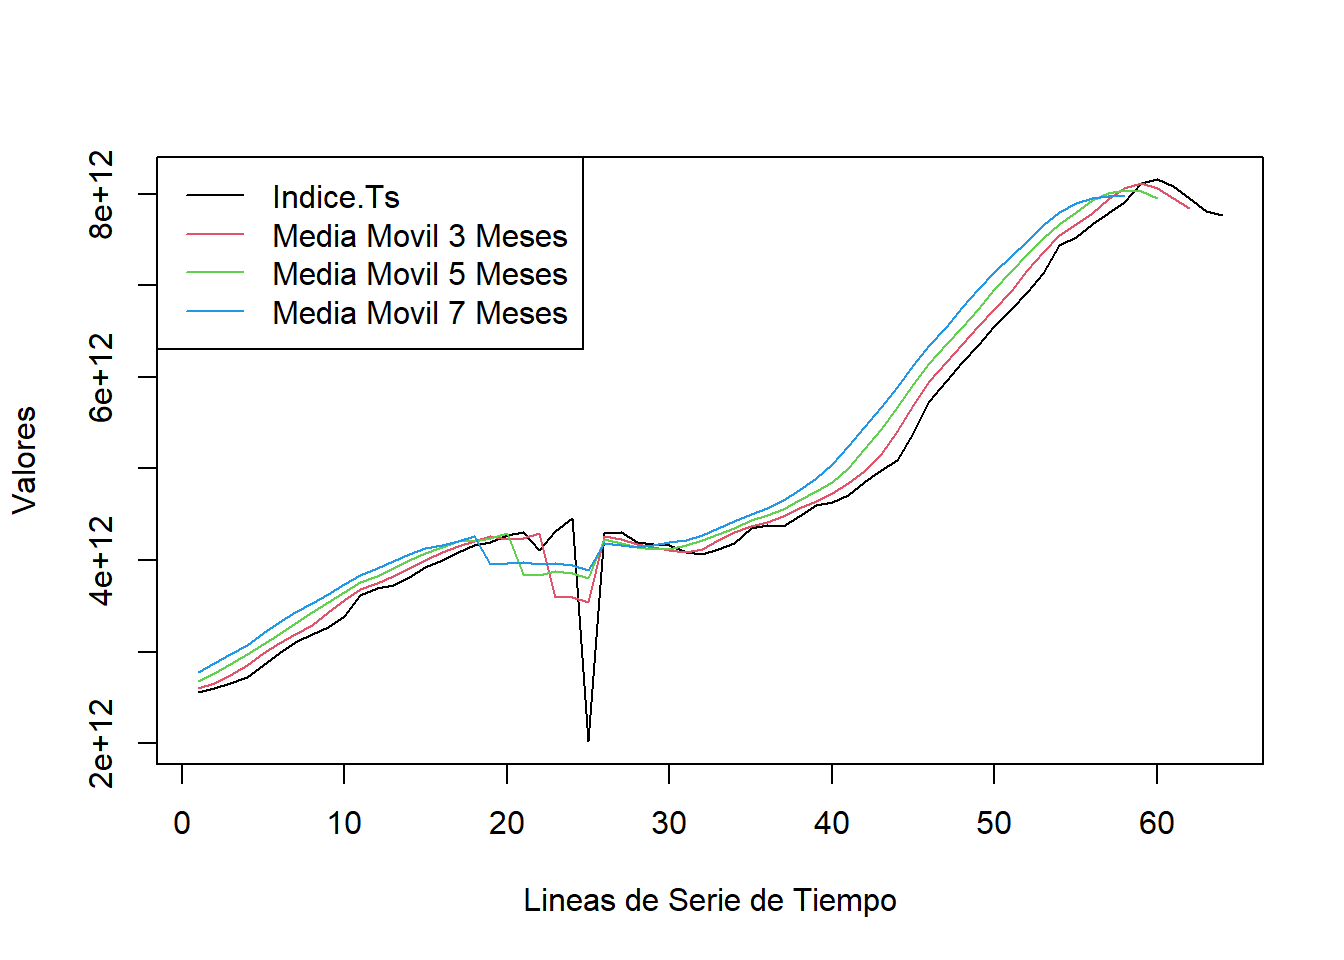
\includegraphics{bookdown-demo_files/figure-latex/unnamed-chunk-7-1.pdf}

\hypertarget{estacionalidad-y-descomposicion}{%
\chapter{Estacionalidad y Descomposicion}\label{estacionalidad-y-descomposicion}}

\hypertarget{Estacion}{%
\section{Estacionalidad}\label{Estacion}}

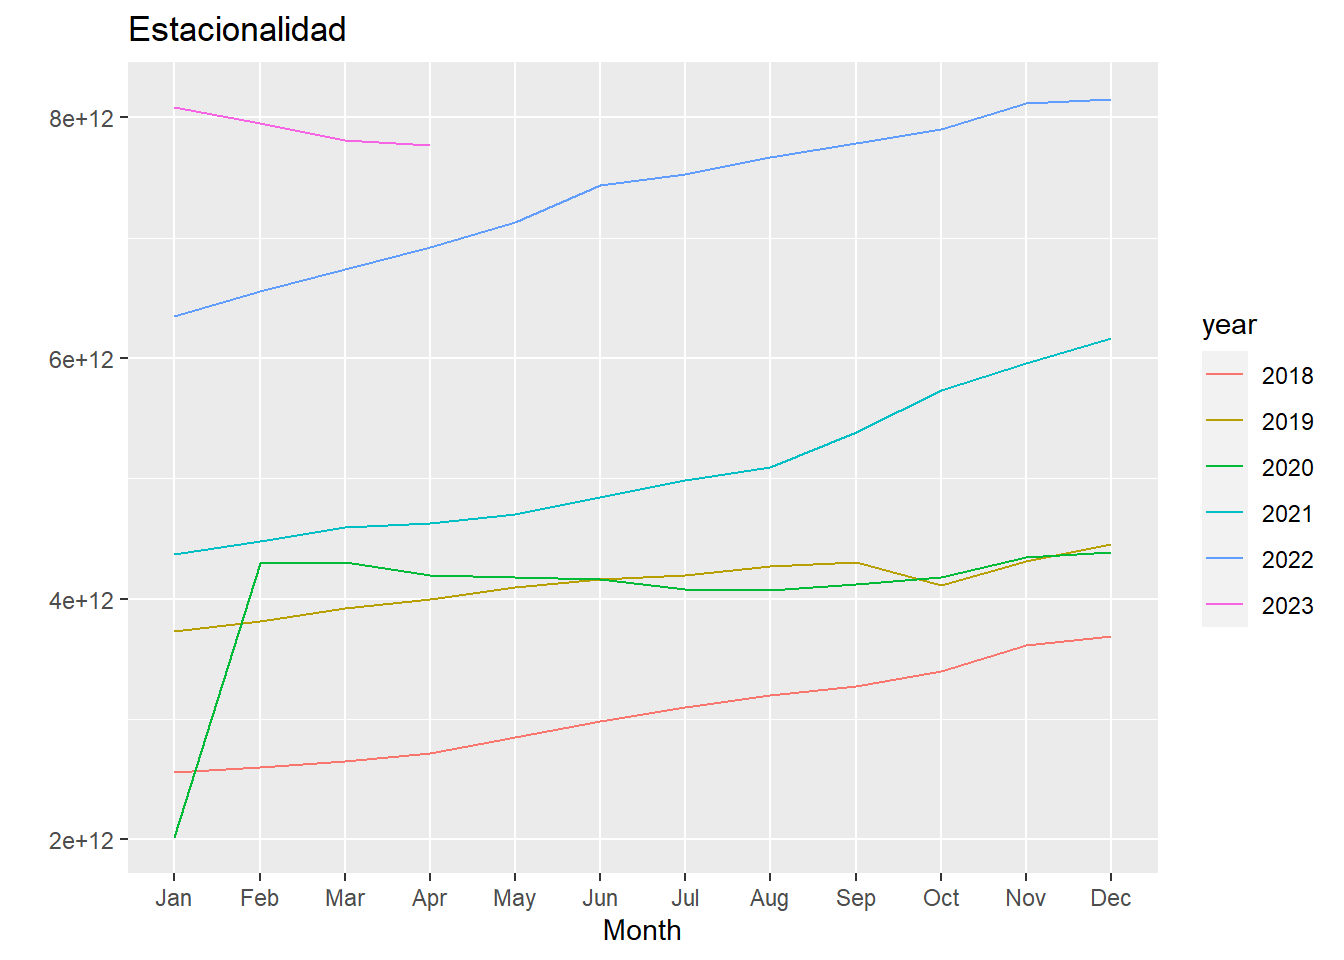
\includegraphics{bookdown-demo_files/figure-latex/unnamed-chunk-8-1.pdf}

\hypertarget{analisis-inicial}{%
\subsection{Analisis Inicial}\label{analisis-inicial}}

Según el análisis de estacionalidad anual, se observa que la utilización de los productos del banco fue moderada en los años 2018 y 2019, tal como se evidencia en las líneas trazadas para esos años. En el 2020, se observa un pico en la utilización que podría indicar un posible error en la recolección de datos. Posteriormente, se observa una pequeña disminución que posiblemente se debió al inicio de la pandemia y la incertidumbre mundial. A partir de septiembre de 2020, se observa un incremento continuo en la utilización para los años 2021 y 2022, posiblemente como resultado de la duración de la pandemia y la crisis económica global.

En el año 2023, se comienza a evidenciar una disminución en la utilización de los productos del banco, lo que podría deberse al alza de las tasas de interés o a un cambio en el comportamiento de los clientes. Es importante mencionar que se requiere un análisis más detallado para determinar las causas precisas de esta disminución.

\hypertarget{descomposicion-del-objeto-y-analisis}{%
\section{Descomposicion del objeto y analisis}\label{descomposicion-del-objeto-y-analisis}}

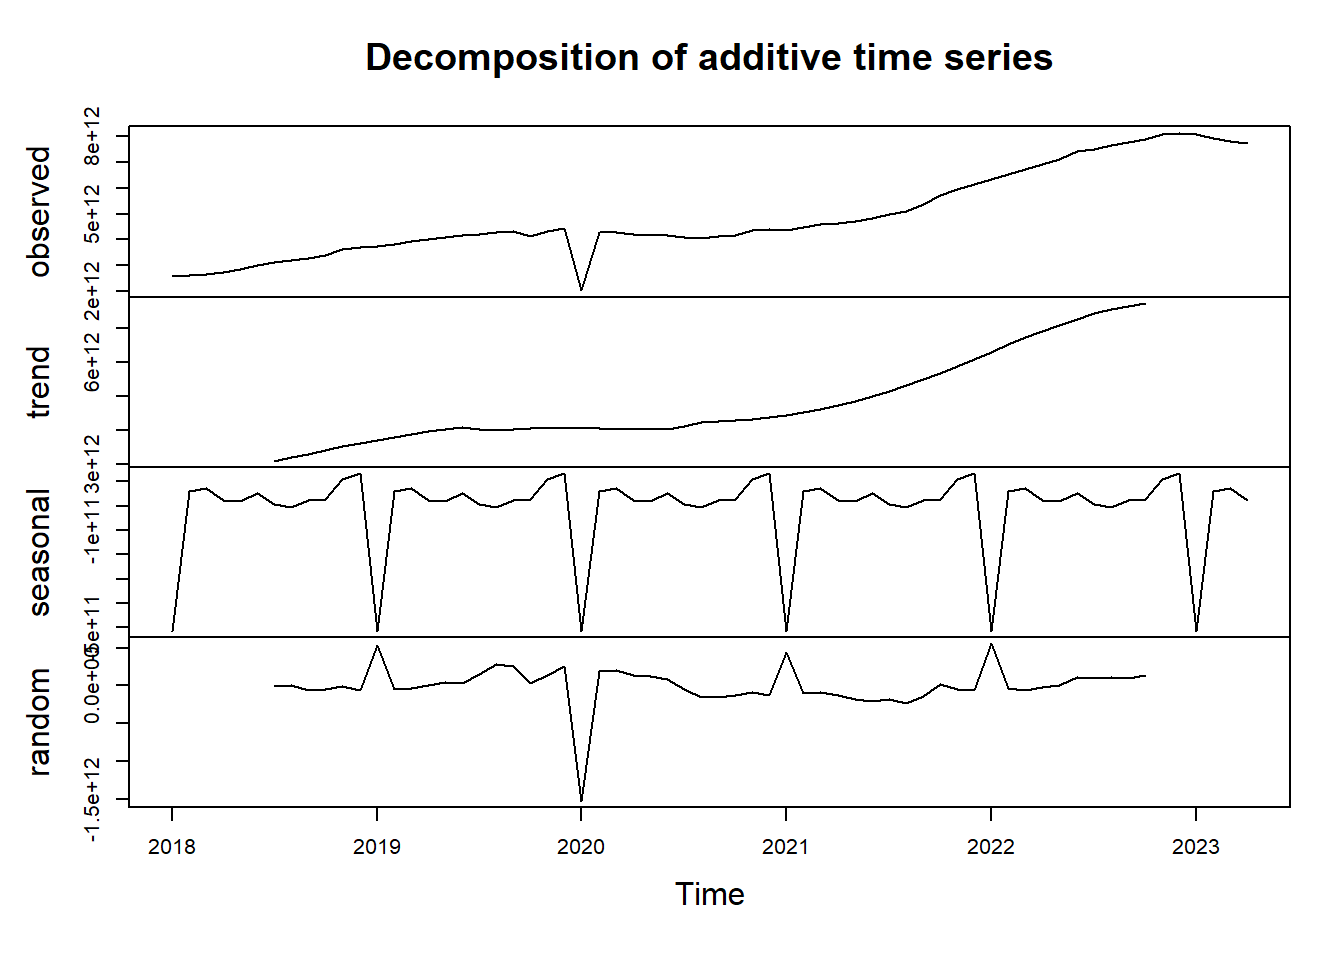
\includegraphics{bookdown-demo_files/figure-latex/unnamed-chunk-9-1.pdf}

A pesar de presentar un patron recurrente en el componente de estacionalidad, se puede observar un trend en la serie de datos. De igual manera el error no se ve aleatorio sino que por el contrario, presenta un patron constante. Dicho esto, vamos a comprobar por medio del Augmented Dickery-Fuller test (adf) la estacionalidad del conjunto de datos.

\hypertarget{prueba-de-estacionalidad}{%
\subsection{Prueba de Estacionalidad}\label{prueba-de-estacionalidad}}

\begin{verbatim}
## 
##  Augmented Dickey-Fuller Test
## 
## data:  indice.ts
## Dickey-Fuller = -1.2017, Lag order = 3, p-value = 0.8984
## alternative hypothesis: stationary
\end{verbatim}

De acuerdo al resultado (p-value \textgreater0.05), debemos aceptar la H0 la cual nos confirma la no-estacionalidad del conjunto. Esto quiere decir que el objeto indice.ts requerira una transformacion para su posterior procesamiento en el modelo.

\hypertarget{autocorrelacion}{%
\subsection{Autocorrelacion}\label{autocorrelacion}}

Ahora veamos si existe autocorrelacion total o parcial.(acf y pacf tests)

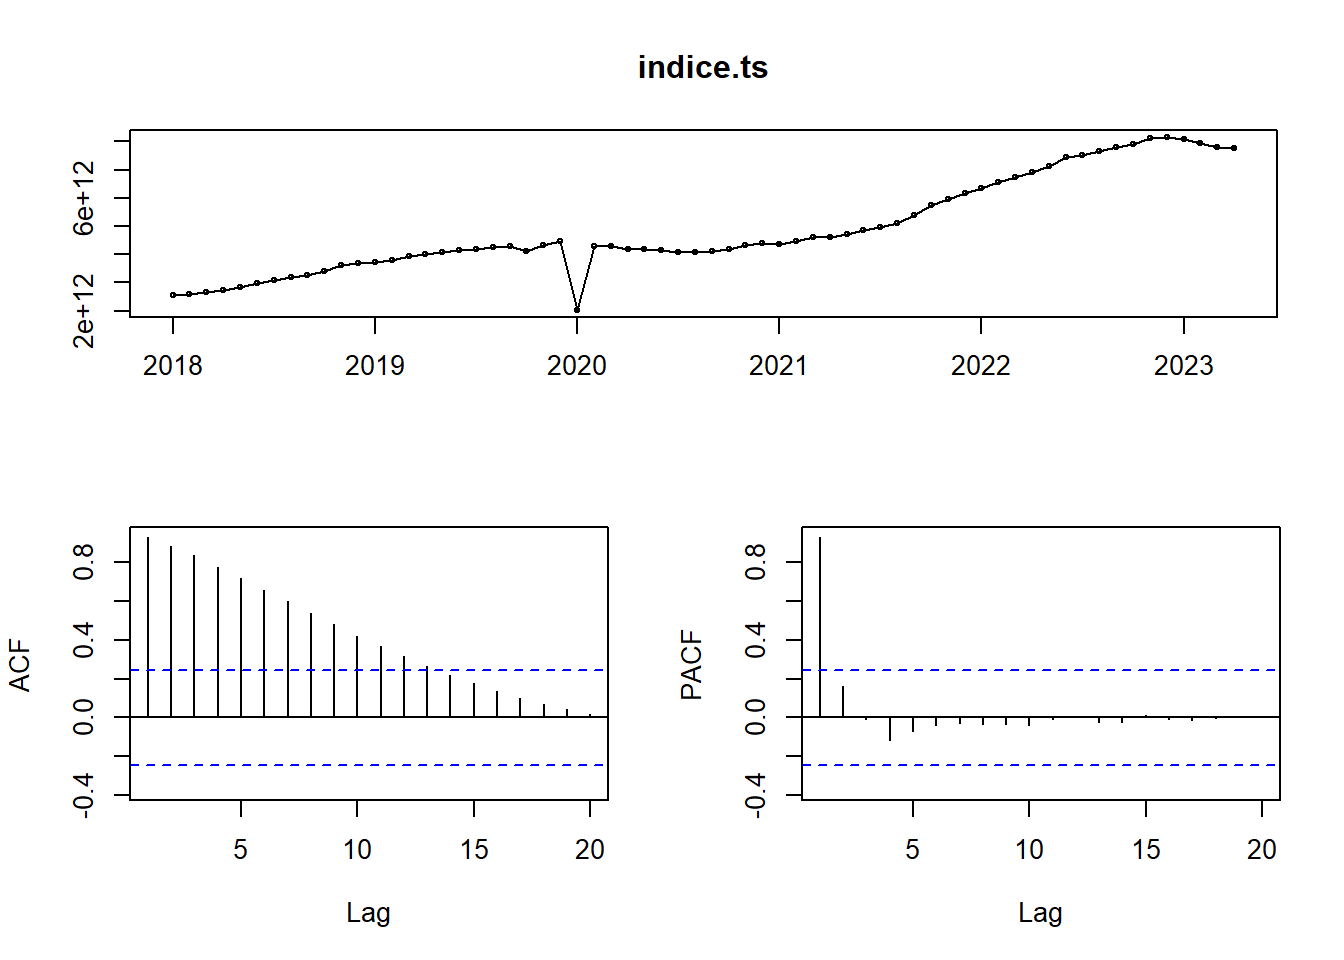
\includegraphics{bookdown-demo_files/figure-latex/unnamed-chunk-11-1.pdf}

Como se puede observar, existe autocorrelacion entre la variable observada lo cual confirma la tendencia en la serie temporal. Por otro lado no evidenciamos autocorrelacion parcial ya que no encontramos picos por fuera del umbral (0.95)

\hypertarget{transformacion}{%
\section{Transformacion}\label{transformacion}}

\begin{verbatim}
## [1] "Ajustamos la estacionalidad de la serie de tiempo por medio del comando seasadj"
\end{verbatim}

\begin{verbatim}
## [1] "Luego removemos la tendencia (trend) con el comando diff"
\end{verbatim}

\begin{verbatim}
## [1] "Grafiquemos la nueva serie de tiempo"
\end{verbatim}

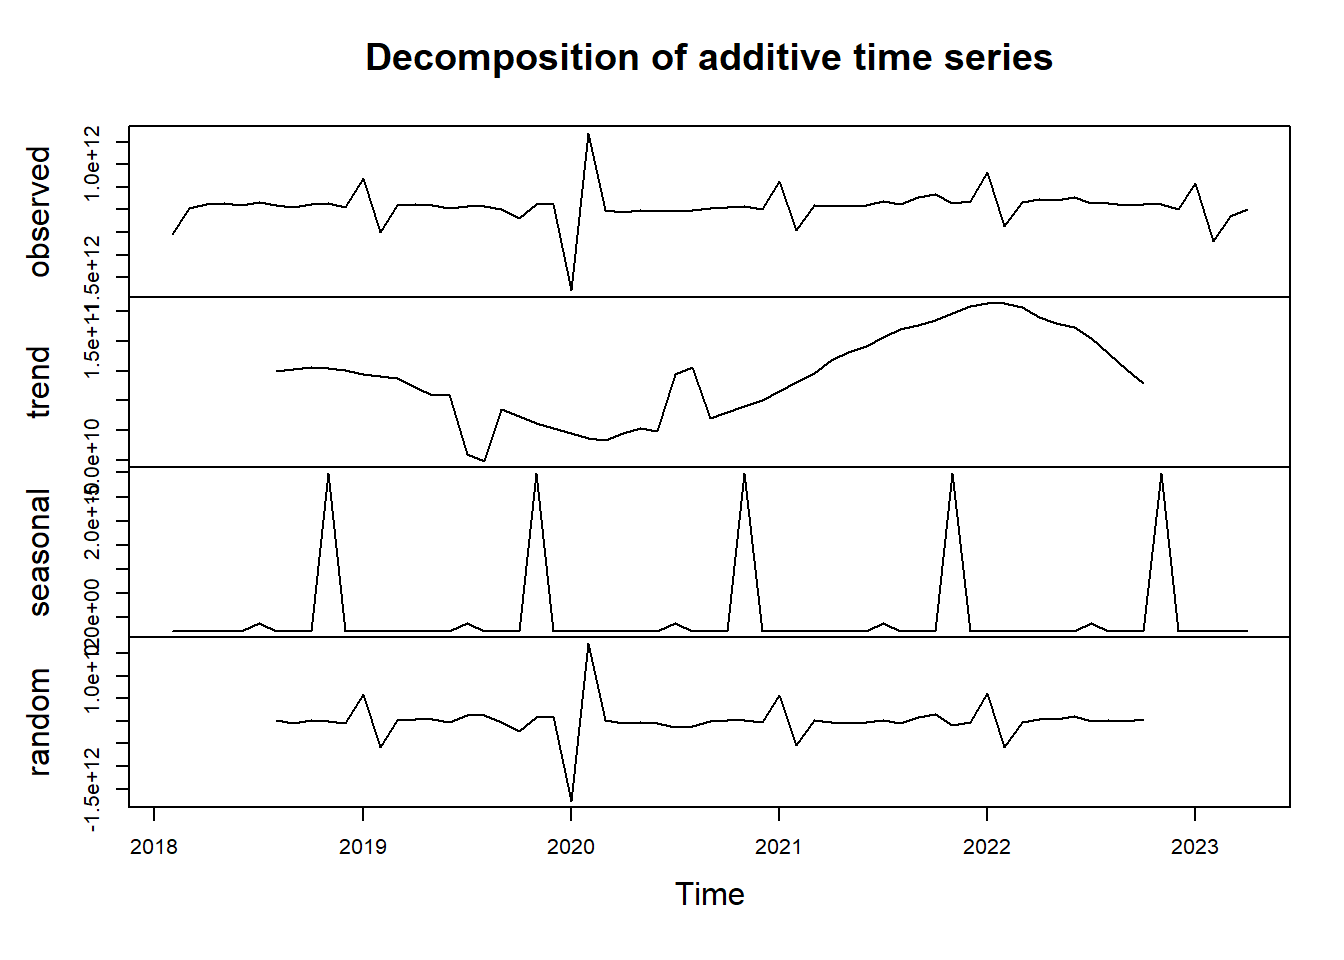
\includegraphics{bookdown-demo_files/figure-latex/unnamed-chunk-12-1.pdf}

\hypertarget{validacion-de-nuestra-nueva-serie-de-tiempo-transformada}{%
\subsection{Validacion de nuestra nueva serie de tiempo transformada}\label{validacion-de-nuestra-nueva-serie-de-tiempo-transformada}}

\begin{verbatim}
## 
##  Augmented Dickey-Fuller Test
## 
## data:  modelo_ts
## Dickey-Fuller = -3.7052, Lag order = 3, p-value = 0.0316
## alternative hypothesis: stationary
\end{verbatim}

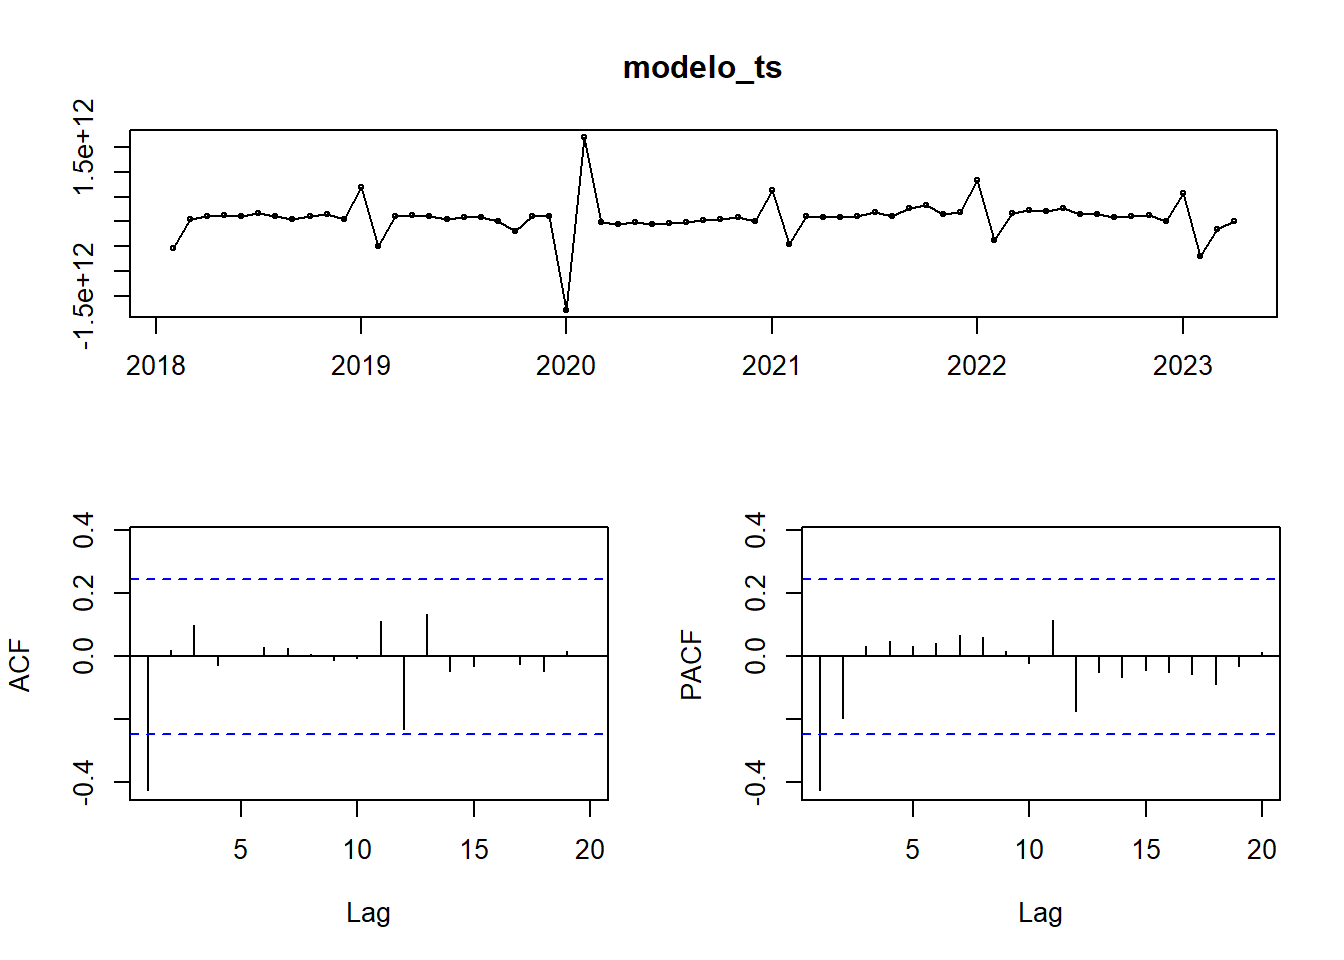
\includegraphics{bookdown-demo_files/figure-latex/unnamed-chunk-13-1.pdf}

se observa que la serie es de tipo estacionaria (p-value=0.0316 \textless{} 0.05), la varianza y la media son de tipo constante, los datos se mueven alrededor de cero (0).

\hypertarget{conclusiones}{%
\section{Conclusiones}\label{conclusiones}}

En conclusión, el análisis de serie de tiempo de la utilización de los productos del banco nos ha permitido identificar patrones y tendencias en su utilización.

A partir del análisis de estacionalidad, se observó que la utilización de los productos del banco ha sido moderada en los años 2018 y 2019, y ha aumentado significativamente en el 2020 y 2021. Además, se evidenció una disminución en la utilización para el año 2023.

La descomposición de la serie de tiempo nos permitió identificar las componentes de tendencia, estacionalidad y error, y su análisis nos ha brindado una mejor comprensión de los patrones y comportamientos observados en la utilización de los productos del banco.

Asimismo, se realizó la diferenciación de la serie de tiempo para eliminar la tendencia y hacer la serie estacionaria. Esto nos permitió obtener una serie de tiempo más homogénea, y por lo tanto, una mejor visualización de las fluctuaciones en la utilización de los productos del banco.Como resultado, la nueva serie de tiempo sera nuestra base para la implementacion de modelos de pronostico de los productos observados.

\hypertarget{methods}{%
\chapter{Methods}\label{methods}}

We describe our methods in this chapter.

Math can be added in body using usual syntax like this

\hypertarget{math-example}{%
\section{math example}\label{math-example}}

\(p\) is unknown but expected to be around 1/3. Standard error will be approximated

\[
SE = \sqrt(\frac{p(1-p)}{n}) \approx \sqrt{\frac{1/3 (1 - 1/3)} {300}} = 0.027
\]

You can also use math in footnotes like this\footnote{where we mention \(p = \frac{a}{b}\)}.

We will approximate standard error to 0.027\footnote{\(p\) is unknown but expected to be around 1/3. Standard error will be approximated

  \[
  SE = \sqrt(\frac{p(1-p)}{n}) \approx \sqrt{\frac{1/3 (1 - 1/3)} {300}} = 0.027
  \]}

\hypertarget{applications}{%
\chapter{Applications}\label{applications}}

Some \emph{significant} applications are demonstrated in this chapter.

\hypertarget{example-one}{%
\section{Example one}\label{example-one}}

\hypertarget{example-two}{%
\section{Example two}\label{example-two}}

\hypertarget{final-words}{%
\chapter{Final Words}\label{final-words}}

We have finished a nice book.

  \bibliography{book.bib,packages.bib}

\end{document}
